\chapter{Introduction}
\label{sec:intro}

\textbf{Large graphs are ubiquitous, and more than a decade of research has investigated how to store and process them efficiently.}
Graphs are a natural data model for relationships between entities in social networks, the World Wide Web, recommendation systems, fraud detection, and biological networks~\cite{ubiquityLargeGraphsVLDB2017}.
Applications now routinely store and analyze graphs with billions of nodes and trillions of edges~\cite{ching2015oneTrillion,besta2020demystifying, lin2018shentu, gupta2024graphscale, zhou2025redtao}.
Nodes and edges may carry \emph{labels} that assign them a type and \emph{properties} modeled as key-value attributes~\cite{besta2020demystifying}; together, the labels and properties give the graph \emph{semantic meaning}, while the nodes and edges alone form the \emph{structure} of the graph.

\textbf{Graph workloads fall into categories analogous to conventional database workloads.}
OLTP queries on graphs resemble their tabular counterparts: a social-network user might retrieve the latest posts on a trending thread. %~\cite{AholeMusk:online}.
Such \emph{interactive} queries are latency-sensitive; real-time applications such as fraud detection in financial networks demand responses within 20\,ms~\cite{qiu2018real}.
Analytical workloads (graph OLAP) require ``whole-graph'' analysis: they operate on the graph structure and typically ignore labels and properties.
For example, Twitter's recommendation teams run PageRank and topic-similarity tasks on the user-follow graph to suggest new accounts to follow~\cite{tang2022taming}.
These two workload classes are served by different systems: graph databases for OLTP and specialized graph processing systems for OLAP.
This dual-silo approach incurs substantial ETL overhead and consistency challenges.

\textbf{Databases are the primary data store for graphs.}
Large-scale graphs originate in relational or key-value databases, and substantial effort has gone into enabling graph analytics within them.
One line of work stores graphs in relational tables and routes analytics to a separate in-memory engine: Facebook's TAO~\cite{bronson2013tao} serves the social graph from MySQL but delegates analytics to offline pipelines; Oracle loads property graphs into PGX, an in-memory graph server, for analysis~\cite{OraclePG,WhatIsOracleSpatialGraph:online,hong2015pgx,welc2013graph,hong2013early}.
A complementary line extends SQL with graph syntax, most notably SQL/Property Graph Query Language (SQL/PGQL)~\cite{duckpgq:online}, but these extensions build only transient in-memory representations and lack persistent graph layouts or transactional mutation support.
When the graph remains in purely relational form, traversals reduce to recursive self-joins whose cost grows with path length~\cite{10.1145/3129246,TransitiveClosureBiskupStiefeling1989}; in every case, analytics still requires a dedicated in-memory engine or an ad-hoc construction step.
None of these approaches provides a single persistent store with analytics-friendly layouts and integrated transactional mutation.

Specialized graph databases such as Neo4j~\cite{neo4j} and ArangoDB~\cite{arangodb} provide schema-oriented organization and a high-level query language.
They handle OLTP workloads well but perform poorly on OLAP tasks.
Graph processing systems such as Pregel~\cite{malewicz2010pregel}, GraphX~\cite{gonzalez2014graphx}, PowerLyra~\cite{powerlyra2019}, GraphChi~\cite{kyrola2012graphchi}, and Ligra~\cite{shun2013ligra} deliver strong OLAP performance but lack OLTP capabilities.
Using them requires extracting the structural graph from the database, transforming it for ingestion, and loading it---a costly ETL pipeline.
\textit{This is the central dichotomy of graph data management}: graph databases provide \emph{persistent graph storage} but are outperformed on OLAP by specialized processing systems, which need a costly ingest and preprocessing phase before analytics can begin.

\textbf{This dichotomy led to the development of Hybrid Graph Transactional and Analytical Processing (HGTAP) systems, such as LiveGraph~\cite{zhu2019livegraph} and GART~\cite{shen2023bridging}.}
LiveGraph stores adjacency lists in a large memory-mapped region (considered harmful~\cite{crotty2022you}) and its analytics-friendly layout delivers robust OLAP performance. 
However, its transaction manager serializes writers, limiting insertion throughput~\cite{libinzhou2025GTX}.
GART constructs an in-memory multi-versioned Compressed Sparse Row (CSR) bounded by main-memory capacity.
Neither system handles the full spectrum of operating conditions that real graph workloads demand.

We studied the graph data management landscape and made five observations:
\begin{enumerate}
  \item \textit{Layout construction time is non-trivial.} A significant amount of time in graph analytics is spent building the in-memory or on-disk data layout, not running the algorithm.
  \item \textit{Transaction management is expensive to build from scratch.} Dynamic graphs require ACID transactions, crash recovery, and concurrency control---substantial engineering that every new system must reimplement.
  \item \textit{No single operating regime suffices.} In-memory systems cannot handle graphs that exceed RAM; out-of-core systems sacrifice speed; distributed processing suffers from severe communication overhead~\cite{mcsherry2015scalability,beamer2016understanding} and poor work balance~\cite{hajidehi2023cuttana}. A practical system must span all three regimes.
  \item \textit{Data layout is the key determinant of performance.} An analytics-friendly persistent layout that preserves scan locality can serve both OLTP and OLAP workloads and can be extended to store full property graphs with typed, columnar storage.
  \item \textit{Most existing systems each target a single operating point}, in-memory or out-of-core processing, static or dynamic graphs, structural or property graphs; few perform well across the entire spectrum.
\end{enumerate}

\textbf{\project{} is a hybrid transactional and analytical graph database that matches the performance of in-memory graph processing systems without data movement or preprocessing, while also delivering high insertion throughput and efficient, columnar property graph storage.}
Rather than building a custom storage engine, \project{} is built on the \wt{}~\cite{WiredTigerDocumentation} key-value store, inheriting a mature transaction manager, write-ahead log, and buffer pool at no additional engineering cost.
\project{} encodes two analytics-friendly structural layouts---adjacency lists and a CSR approximation---as sorted key ranges in \wt{}, producing sequential scan performance for analytics, and extends them with a typed property storage layer supporting both embedded and columnar modes.
Insertion throughput scales near-linearly to 72 threads, sustaining up to 1.48\,M edges/sec on the write-optimized layout (\autoref{fig:dynamic-scaling}, while property-mutation latencies are three to four orders of magnitude lower than Neo4j~\cite{neo4j} and JanusGraph~\cite{janusgraph}.
% \preliminary{Concurrent insertion and analytics results show that analytics latency remains competitive at moderate write ratios, with \project{} sustaining $1.8\times$ the mixed-workload write throughput of LiveGraph at the balanced operating point.}
A programmer uses \project{} through a library API that exposes read-only snapshot iterators over neighborhoods and properties to express analytics tasks. We modified the GAP Benchmark Suite (GAPBS)~\cite{beamer2015gap} to use this API and show that \project{}'s end-to-end analytics performance matches in-memory systems while scaling to out-of-core graphs.
\autoref{fig:fg-spider} summarizes these results: \project{} delivers robust performance across the entire spectrum of operating conditions, where every other system we evaluate falters significantly in two or more regimes.
A system purpose-built for a single regime can outperform \project{} in that niche; Teseo significantly outperforms us on dynamic graph ingest and update operations.
That said, no other system we evaluate matches its breadth while providing full transactional guarantees.
\textbf{Our contributions} are as follows.
\begin{itemize}
  \item The design of \project{}, a hybrid graph database built on \wt{} that unifies OLTP and OLAP graph workloads in a single persistent store without ETL or preprocessing.
  \item An analysis of analytics-friendly data layouts and a demonstration of how adjacency-list and CSR-like representations can be encoded as sorted key ranges in a key-value store to preserve scan locality.
  \item A typed property storage layer with embedded and columnar modes that achieves property-mutation latencies three to four orders of magnitude lower than that of Neo4j, JanusGraph, and ArangoDB.
  \item Efficient, read-only neighborhood iterators on graph snapshots, with a flexible partitioning strategy that splits work between threads by vertex count or edge count.
  \item An evaluation showing that \project{} matches the analytics performance of in-memory and out-of-core graph processing systems, scales insertion throughput near-linearly, and delivers the transactional performance of in-memory dynamic graph containers.
\end{itemize}

\begin{figure}[t]
  \centering
  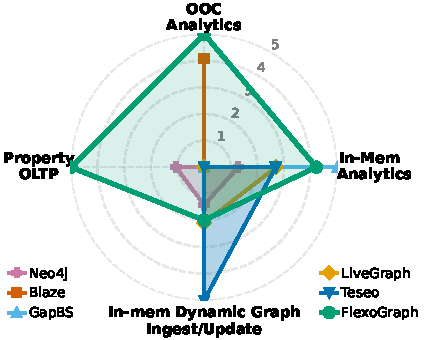
\includegraphics[scale=0.75]{content/fig/spider_chart_v2.pdf}
  \caption{\project{} delivers robust performance across the entire spectrum of operating conditions common in graph data management. Each axis represents a workload class; points closer to the boundary indicate better performance relative to the best system in that class.}
  \label{fig:fg-spider}
\end{figure}